% Charlotte Geiger - Manuel Lippert - Leonard Schatt
% Physikalisches Praktikum

% Teilauswertung 2

\section{Nutation}

Bei genauer Beobachtung des Kreisels kann man neben der Präzessionsbewegung erkennen, dass die Kreiselachse nicht komplett ruhig um die Senkrechte läuft, sondern viel mehr kleine Rotationen auf der Bahn der Präzession vollführt. Das ist das Phänomen der Nutation.\\
Um diese Nutation des Kreisels zu untersuchen, bestimmt man die Nutationsfrequenz des momentfreien Kreisels als Funktion von $\omega_3$. Damit es gut darzustellen und auszuwerten ist, betrachtet man $w_3$ im Bezug zu dem Quotienten $\frac{w_n}{w_3}$, wobei dieser fortan als $\omega_N$ bezeichnet wird. \\
Um die Frequenz in die Winkelgeschwindigkeit umzurechnen, muss man die Frequenz mit $2\pi$ multiplizieren $(w =2\pi\cdot f)$.\\
Der Fehler des Stroboskops wird abgeschätzt mit $u_{f_3}=0.25~\text{Hz}$, da der Ablesefehler für die verwendete Messmethode zu optimistisch ist. \\
Auch bei der Zeitmessung muss der Fehler mitbetrachtet werden, dabei ist einmal der Ablesefehler $u_a=0.01~\text{s}$ der Stoppuhr und die Reaktionszeit der Messperson. Aus dem Versuch MES aus dem Sommersemester 2020 wissen wir, dass die Messperson eine Reaktion von $t_{react}=(0.188\pm0.013)~\text{s}$ besitzt. Damit können wir den Fehler der Zeitmessung mit $u_t=0.20~\text{s}$ angeben. \\
Des Weiteren wird der Mittelwert der Zeiten aus den beiden Messreihen gebildet und dieser durch 10 geteilt (wegen 10 Umdrehungen) wird, um die Rotationsdauer $T_n$ zu erhalten. Daraus folgen die Formeln der Fehler mit dem \textbf{Fehlerfortpflanzungsgesetz}:
\begin{gather}
    \omega_3^i=2\pi\cdot f_3^i  \tab \omega_n^i = \frac{2\pi}{T_n^i}\\
    t_n^i = \frac{t_{n_1}^i+t_{n_2}^i}{2}\tab u_{t_n} = \frac{1}{2}\sqrt{u_t^2+u_t^2}=\frac{u_t}{\sqrt{2}}\\
    T_n^i=\frac{t_n^i}{10} \tab u_{T_n} = \frac{1}{10}\sqrt{10u_{t_n}^2} = \frac{u_{t_n}}{\sqrt{10}}\\[0.3mm]
    \omega_N^i=\frac{\omega_n^i}{\omega_3^i} = \frac{1}{T_n^i f_3^i} 
    \tab u_{\omega_N^i} = \sqrt{\left(\frac{u_{T_n}}{{T_n^i}^2f_3^i}\right)^2+\left(\frac{u_{f_3}}{T_n^i{f_3^i}^2}\right)^2} 
\end{gather}
Um das Verhältnis von $\omega_3$ im Bezug zu $\omega_N$ tabellarisch aufzutragen, muss man auf das Vorzeichen achten. Aus den Eulerschen Gleichungen für den momentfreien, symmetrischen Kreisel wurde folgendes im Skript angegeben:
\begin{align}
    \omega_N^i = \frac{J_3 - J_1}{J_1} = \text{konstant}
\end{align}
Da wir aber nur noch einen symmetrischen Kreisel mit $J_1 = J_2$ und $J_3<J_1$ betrachten, ist das konstante Verhältnis negativ, was mit einem - Zeichen bei $\omega_N$ verdeutlicht wird. 
\newpage
\begin{center}
    \captionof{table}{Nutationswerte}
    \begin{tabular}{gcccccccc}
        \rowcolor[rgb]{ .741,  .843,  .933}{} &     $t_n/\text{s}$ &   $u_{t_n}/\text{s}$ &     $T_n/\text{s}$ &   $u_{T_n}/\text{s}$ &      $\omega_3/\frac{1}{\text{s}}$ &    $\omega_n/\frac{1}{\text{s}}$ &      $\omega_N$ &    $u_{\omega_N}$ \\
        1  &  61.33 &  0.14 &  6.13 &  0.04 &   62.83 &  1.02 & -0.0163 &  0.0004 \\
        2  &  59.17 &  0.14 &  5.92 &  0.04 &   65.97 &  1.06 & -0.0161 &  0.0004 \\
        3  &  58.32 &  0.14 &  5.83 &  0.04 &   69.12 &  1.08 & -0.0156 &  0.0004 \\
        4  &  51.33 &  0.14 &  5.13 &  0.04 &   75.40 &  1.22 & -0.0162 &  0.0004 \\
        5  &  49.25 &  0.14 &  4.92 &  0.04 &   81.68 &  1.28 & -0.0156 &  0.0003 \\
        6  &  45.16 &  0.14 &  4.52 &  0.04 &   87.96 &  1.39 & -0.0158 &  0.0003 \\
        7  &  40.66 &  0.14 &  4.07 &  0.04 &   94.25 &  1.55 & -0.0164 &  0.0003 \\
        8  &  37.88 &  0.14 &  3.79 &  0.04 &  100.53 &  1.66 & -0.0165 &  0.0003 \\
        9  &  36.01 &  0.14 &  3.60 &  0.04 &  106.81 &  1.74 & -0.0163 &  0.0003 \\
        10 &  34.45 &  0.14 &  3.44 &  0.04 &  113.10 &  1.82 & -0.0161 &  0.0003 \\
        11 &  32.96 &  0.14 &  3.30 &  0.04 &  119.38 &  1.91 & -0.0160 &  0.0003 \\
        12 &  30.97 &  0.14 &  3.10 &  0.04 &  125.66 &  2.03 & -0.0161 &  0.0003 \\
    \end{tabular}
\end{center}
\begin{figure}[ht]
    \centering
    \caption{$w_N$ Histogramm}
    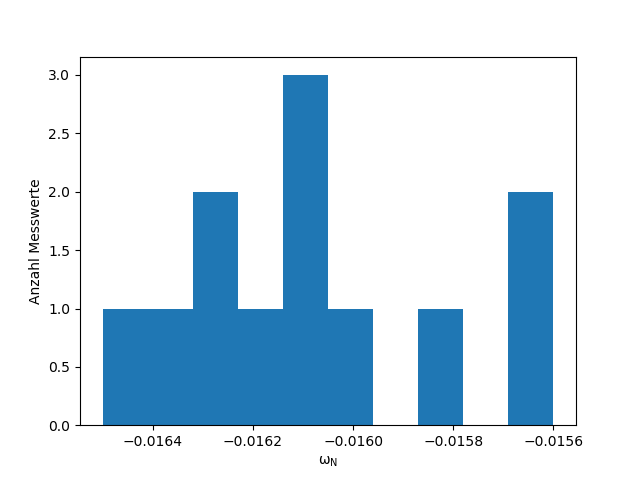
\includegraphics[scale=0.6]{62-Hist.png}
\end{figure}
Nun wird die Konstante durch den Mittelwert der berechneten Verhältnisse berechnet.
\begin{align}   
    \overline{\omega_N} = \frac{1}{M}\sum_{i=1}^{M}\omega_N^i \tab u_{\overline{\omega_N}}= \frac{1}{M}\sqrt{\sum_{i=1}^{M}u_{\omega_N^i}^2} \tab M:\text{Anzahl der Werte}
\end{align}
Da aber die Werte von $\omega_N$ sehr nah beieinanderliegen wird der Fehler des Mittelwerts vernachlässigt und der Fehler von $\overline{\omega_N}$ als Mittelwert der Fehler von $\omega_N$ abgeschätzt.
\begin{align*}
    \Rightarrow\boxed{\overline{\omega_N}=(-0.01608\pm0.00097)}
\end{align*}
\newpage
\begin{figure}[ht]
    \centering
    \caption{$\omega_3-\omega_N$ Diagramm}
    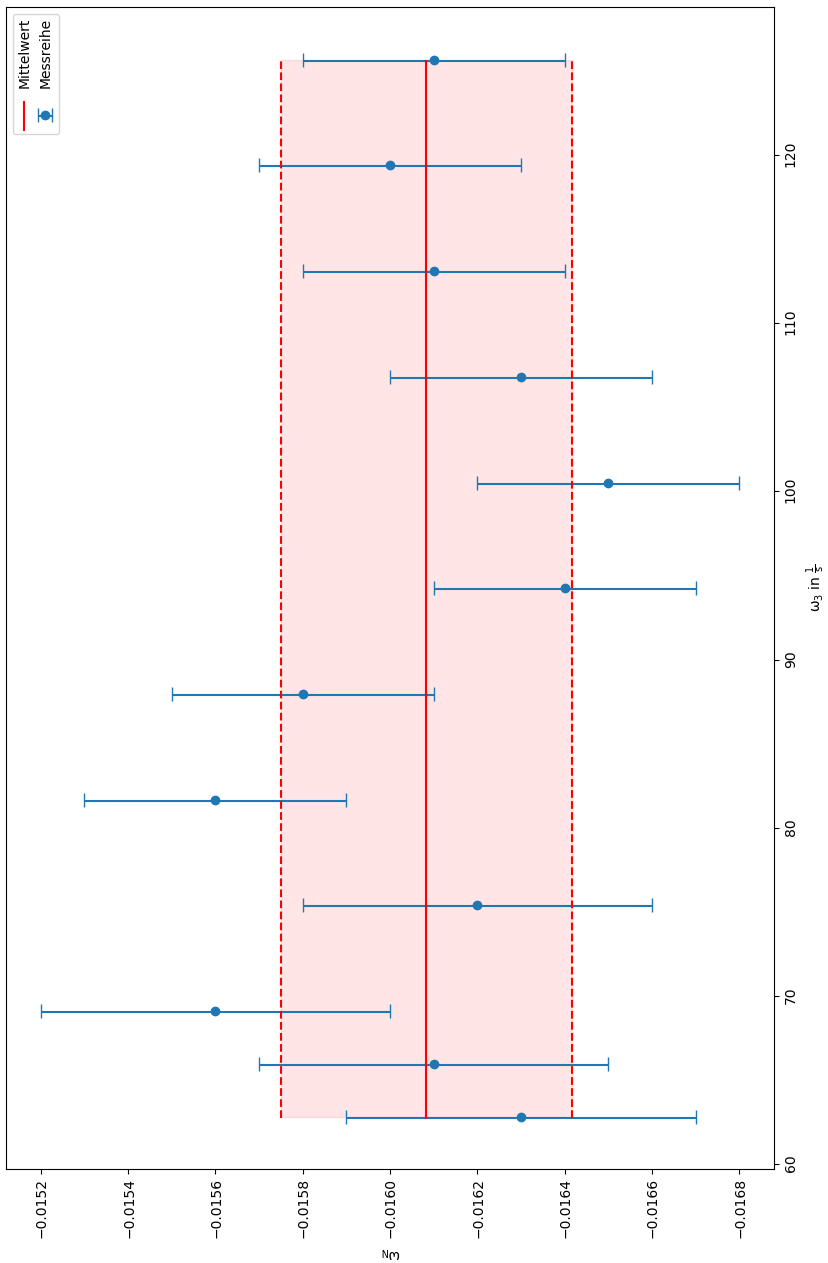
\includegraphics[scale=0.6]{62-Nutation.png}
\end{figure}